\section{锁的原理}
\subsection{LockSupport}

LockSupport 是个工具类,没有公有的构造函数。它的主要作用是挂起和唤醒线程,是创建锁和其他同步类的基础:

\begin{Java}
public class LockSupport {
    private static final Unsafe U = Unsafe.getUnsafe();
}
\end{Java}

LockSupport类与每个使用它的线程都会关联一个许可证,在默认情况下调用 LockSupport 类的方法的线程是不持有许可证的。

\subsubsection*{park() 方法}

park 系方法是 LockSupport 的核心方法,本质上是调用 Unsafe 的 park() 方法,具体方法实现是不可知的:

\begin{Java}
public static void park() {
    U.park(false, 0L);
}
\end{Java}

如果调用park方法的线程已经拿到了与LockSupport关联的许可证,则调用LockSupport.park()时会马上返回,否则调用线程会被禁止参与线程的调度,也就是会被阻塞挂起。

在其他线程调用 unpark(Thread thread)方法并且将当前线程作为参数时,调用park方法而被阻塞的线程会返回。另外,如果其他线程调用了阻塞线程的interrupt()方法,设置了中断标志或者线程被虚假唤醒,则阻塞线程也会返回。所以在调用park方法时最好也使用循环条件判断方式。

需要注意的是,因调用park()方法而被阻塞的线程被其他线程中断而返回时并不会抛出InterruptedException异常。

\subsubsection*{unpark(Thread thread) 方法}

\begin{Java}
public static void unpark(Thread thread) {
    if (thread != null)
        U.unpark(thread);
}
\end{Java}

当一个线程调用unpark时,如果参数thread线程没有持有thread与LockSupport类关联的许可证,则让thread线程持有。如果thread之前因调用park()而被挂起,则调用unpark后,该线程会被唤醒。如果thread之前没有调用park,则调用unpark方法后,再调用park方法,其会立刻返回。

park方法返回时不会告诉你因何种原因返回,所以调用者需要根据之前调用park方法的原因,再次检查条件是否满足,如果不满足则还需要再次调用park方法。例如:

\begin{Java}
// 调用 park 方法,挂起自己,只有被中断才退出
while(!Thread.currentThread().isInterrupted) {
    LockSupport.park();
}
\end{Java}

\subsubsection*{其他 park 系方法}

park 系方法还有几个参数:
\begin{itemize}
    \item long nanos: 如果没有拿到许可证,则调用线程会被挂起nanos时间后修改为自动返回。
    \item long deadline: 和 nAQS 类似,nanos 是从当前时间开始等待多久,deadline 是等待到什么时间。
    \item Object blocker: 当线程在没有持有许可证的情况下调用park方法而被阻塞挂起时,这个blocker对象会被记录到该线程内部,该对象通常为 this,即调用线程的类本身。
\end{itemize}。

\subsection{AQS 抽象同步队列}
\subsubsection{AQS 基础介绍}

AbstractQueuedSynchronizer抽象同步队列简称AQS,它是实现同步器的基础组件,并发包中锁的底层就是使用AQS实现的。开过过程中几乎不会直接调用 AQS,理解即可。

\begin{Java}
public abstract class AbstractQueuedSynchronizer extends AbstractOwnableSynchronizer implements java.io.Serializable
\end{Java}

\begin{center}
    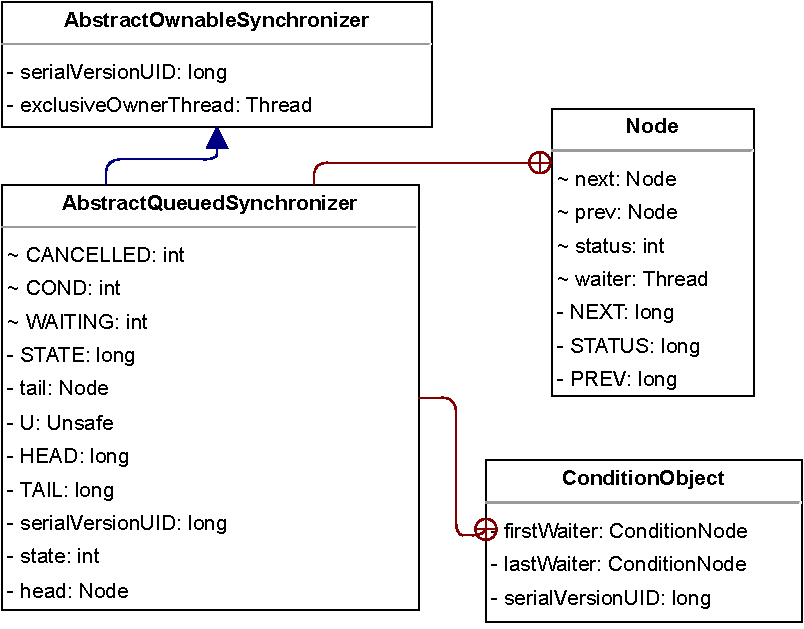
\includegraphics[width=0.6\linewidth]{../../../Images/AQS.pdf}
\end{center}

AQS 核心思想是,如果被请求的共享资源空闲,则将当前请求资源的线程设置为有效的工作线程,并且将共享资源设置为锁定状态。如果被请求的共享资源被占用,那么就需要一套线程阻塞等待以及被唤醒时锁分配的机制,这个机制 AQS 是用 CLH(虚拟的双向队列) 队列锁实现的,即将暂时获取不到锁的线程加入到队列中。

AQS 是一个 FIFO 双向队列,他有两个关键的内部类,他们的关键属性如下:
\begin{itemize}
    \item Node: 队列元素(没有公有方法)
    \begin{itemize}
        \item Thread waiter: 存放进入 AQS 队列的线程。Node 有两个子类用于标记线程阻塞原因:
        \begin{itemize}
            \item SharedNode: 标记线程是获取共享资源时被挂起进入 AQS 队列。
            \item ExclusiveNode: 标记线程时获取独占资源时被挂起后进入 AQS 队列。
        \end{itemize}
        \item int status: 用于记录当前线程等待状态,提供了三个常量:
        \begin{itemize}
            \item WAITING: 普通的等待状态。
            \item CANCELLED: 线程被取消。
            \item COND: 条件等待。
        \end{itemize}
    \end{itemize}
    \item ConditionObject: 条件变量,加强版 notify 和 wait 操作,下文细嗦。
    \begin{itemize}
        \item ConditionNode: 继承自 Node 的内部类,记录等待节点顺序。
        \item firstWaiter/lastWaiter: 用于记录第一和最后一个等待线程节点。
    \end{itemize}
\end{itemize}

AQS 最关键的属性是 state,不同的锁对其有不同的用法:
\begin{itemize}
    \item ReentrantLock: 表示当前线程获取锁的可重入次数。
    \item ReentrantReadWriteLock: 高于 16 表示读状态,低于16表示可重入次数。
    \item semaphore: 当前可用信号数。
    \item CountDownlatch: 计数器当前的值。
\end{itemize}

对于AQS来说,线程同步的关键是对状态值state进行操作。根据state是否属于一个线程,操作state的方式分为独占方式和共享方式。AQS 通过 acquire 系方法获取资源,release 系方法释放资源。共享和独占资源对应的方法不同:

\begin{itemize}
    \item 使用独占方式获取的资源是与具体线程绑定的,就是说如果一个线程获取到了资源,就会标记是这个线程获取到了,其他线程再尝试操作state获取资源时会发现当前该资源不是自己持有的,就会在获取失败后被阻塞。
    \item 对应共享方式的资源与具体线程是不相关的,当多个线程去请求资源时通过CAS方式竞争获取资源,当一个线程获取到了资源后,另外一个线程再次去获取时如果当前资源还能满足它的需要,则当前线程只需要使用CAS方式进行获取即可。
\end{itemize}

\subsubsection*{获取与释放资源}

在前面我们已经了解到,state 属性值的具体含义由子类赋予,因此与之相关的操作也全部由子类负责,父类仅提供接口。

在独占模式下,获取与释放资源有如下过程:

\begin{itemize}
    \item 获取资源: acquire(int arg) 方法。
\begin{Java}
public final void acquire(int arg) {
    if (!tryAcquire(arg))   // 具体实现由子类提供
        acquire(null, arg, false, false, false, 0L);
}
\end{Java}
    \begin{itemize}
        \item 首先会使用 tryAcquire(arg) 方法尝试获取资源,具体是设置状态变量 state 的值。
        \item 如果成功,直接返回。
        \item 如果失败,将当前线程封装为 ExclusiveNode 插入到 AQS 队列的尾部,调用 LockSupport.park 方法挂起自己。
    \end{itemize}
    \item 释放资源: release(int age) 方法。
\begin{Java}
public final boolean release(int arg) {
    if (tryRelease(arg)) {  // 同样由子类实现
        signalNext(head);   // 激活第一个被阻塞的线程并尝试获取资源
        return true;
    }
    return false;
}
\end{Java}
    \begin{itemize}
        \item 首先尝试使用tryRelease操作释放资源,具体也是操作 state 的值。
        \item 调用 LockSupport.unpark 激活 AQS 队列里被阻塞的第一个线程。
        \item 被激活的线程调用 acquire 方法,尝试获取资源。
    \end{itemize}
\end{itemize}

在共享模式下,获取与释放资源的操作类似,不过在获取资源失败后会线程会被封装为 SharedNode 插入队尾。

除了上述介绍的方法外,还需要重写 isHeldExclusively()方法,来判断锁是否已经被持有。

AQS 还提供了带 Interruptibly 后缀的 acquire 方法,不带Interruptibly关键字的方法的意思是不对中断进行响应,那么该线程不会因为被中断而抛出异常,而带Interruptibly关键字的方法要对中断进行响应。

虚拟的双向队列不存在队列实例,仅存在结点之间的关联关系,因此 AQS 每次入队操作实质上都是将线程封装成 Node 节点后添加进双向链表的操作。

\subsubsection{条件变量的支持}

正如 notify 和 wait 是配合 synchronized 内置锁实现线程间同步,ConditionObject(条件变量)的 signal 和 await 方法也是用来配合锁(AQS 实现的锁)实现线程同步的。不同点在于 synchronized 是共享线程独占锁,而 AQS 的锁可以对应多个条件变量。

\begin{Java}
public class ConditionObject implements Condition, java.io.Serializable
\end{Java}

在调用共享变量的notify和wait方法前必须先获取该共享变量的内置锁,同理,在调用条件变量的signal和await方法前也必须先获取条件变量对应的锁。

下面看一个 ReentrantLock(AQS 实现) 例子:

\begin{Java}
ReentrantLock lock = new ReentrantLock();   // 创建一个 ReentrantLock 锁
Condition condition = lock.newCondition();  // 创建一个条件变量

lock.lock();    // 获取锁
try {
    System.out.println("begin wait");
    condition.await();      // 阻塞挂起当前线程
    System.out.println("end wait");
} catch (Exception ex) {
    ex.printStackTrace();
} finally {
    lock.unlock();      // 释放锁
}
\end{Java}

这里的一些操作解释如下:
\begin{itemize}
    \item Lock 对象: 等价于 synchronized 加上共享变量。
    \item lock.lock(): 等价于进入 synchronized 块尝试获取锁。
    \item lock.unlock(): 等价于退出 synchronized 块释放锁。
    \item await() 方法: 等价于 Object 的 wait() 方法。
    \item signal() 方法: 等价于 Object 的 notify() 方法。
\end{itemize}

当线程调用条件变量的 await() 方法时(先调用 lock() 方法),在内部会构造一个 ConditionNode 型的 node 节点,然后插入节点,之后当前线程会释放获取的锁并被阻塞挂起。await() 方法的部分源码如下:

\begin{Java}
public final void await() throws InterruptedException {
    if (Thread.interrupted())
        throw new InterruptedException();
    // 创建新的节点
    ConditionNode node = new ConditionNode();
    // 释放当前线程获取的锁,插入节点
    int savedState = enableWait(node);
    // 阻塞挂起当前线程
    LockSupport.setCurrentBlocker(this);
    ......
}
\end{Java}

继续深入看一下如何获取锁并插入节点:

\begin{Java}
private int enableWait(ConditionNode node) {
    if (isHeldExclusively()) {  // 锁被持有
        node.waiter = Thread.currentThread();   // 将线程装入节点
        node.setStatusRelaxed(COND | WAITING);
        ConditionNode last = lastWaiter;
        if (last == null)
            firstWaiter = node;
        else
            last.nextWaiter = node;     
        lastWaiter = node;              // 插入节点完成,注意这是一个单向队列
        int savedState = getState();
        if (release(savedState))
            return savedState;
    }
    node.status = CANCELLED; // 获取锁失败
    throw new IllegalMonitorStateException();
}
\end{Java}

当多个线程同时调用lock.lock()方法获取锁时,只有一个线程获取到了锁,其他线程会被转换为Node节点插入到lock锁对应的AQS阻塞队列里面,并做自旋CAS尝试获取锁。

如果获取到锁的线程又调用了对应的条件变量的await()方法,则该线程会释放获取到的锁,并被转换为Node节点插入到条件变量对应的条件队列\footnote{条件队列: \url{https://blog.csdn.net/weixin_33188789/article/details/114869897}}里面。

当另外一个线程调用条件变量的signal()或者signalAll()方法时,会把条件队列里面的一个或者全部Node节点移动到AQS的阻塞队列里面,等待时机获取锁。

一个锁对应一个 AQS 阻塞对象,对应多个条件变量。下图解释了条件队列与 AQS 阻塞队列的关系:

\begin{figure}[H]
    \centering
    \small
    \begin{tikzpicture}[scale = 1]
        \node[draw] (lock) at (0,0) {Lock}; 
        \foreach \y in {1,0,-1} {
            \node[draw] (Condition-\y) at (3,\y) {Condition};
            \node[draw] (条件队列-\y) at (6,\y) {条件队列};
            \draw[-Stealth] (Condition-\y) -- (条件队列-\y);
            \draw[-Stealth] (lock) -- (Condition-\y);
        }
        \node [draw,above,text width=1em] (AQS) at (-2,-2) {A Q S 阻塞队列};
        \draw [-Stealth] (lock) -- (AQS);
    \end{tikzpicture}
    \caption{条件队列}
    \label{fig:条件队列}
\end{figure}

\subsection{ReentrantLock 独占锁}

\subsubsection*{Lock 接口与 ReentrantLock 基础}

所有锁都需要实现 Lock 接口,它提供了最基础的方法:
\begin{itemize}
    \item void lock(): 获取锁。
    \item void lockInterruptibly(): 获取锁,被中断则抛异常。
    \item boolean tryLock(): 尝试获取锁,不会引起阻塞。
    \item boolean tryLock(long time, TimeUnit unit): 在一段时间内尝试获取锁。
    \item void unlock(): 释放锁。
    \item Condition newCondition(): 获取条件变量。
\end{itemize}

ReentrantLock 是可重入的独占锁,同时只能有一个线程可以获取该锁,其他获取该锁的线程会被阻塞而被放入该锁的AQS阻塞队列里面。

\begin{Java}
public class ReentrantLock implements Lock, java.io.Serializable
\end{Java}

ReentrantLock 只有一个功能性成员变量: Sync sync,Sync 继承自 AQS 重写了一些方法。ReentrantLock 本质上还是使用 AQS 来实现的,可以根据参数决定它是一个公平锁还是非公平锁。

\begin{Java}
public ReentrantLock() {
    sync = new NonfairSync();
}

public ReentrantLock(boolean fair) {
    sync = fair ? new FairSync() : new NonfairSync();
}
\end{Java}

其中 NonfairSyn 和 FairSync 继承自 Sync,分别实现了锁的非公平与公平策略。

在这里,state 表示线程获取锁的可重入次数,默认情况下,state = 0 表示当前锁没有被任何线程持有。当一个线程第一次获取该锁时会尝试使用 CAS 设置 state 值为1,如果 CAS 成功则当前线程获取了该锁,然后记录该锁的持有者为当前线程。在该线程没有释放锁的情况下第二次获取该锁后,状态值被设置为2,这就是可重入次数。在该线程释放该锁时,会尝试使用CAS让状态值减1,如果减1后状态值为0,则当前线程释放该锁。

\subsubsection*{公平锁与非公平}

我们说过 AQS 没有提供可用的 tryAcquire 方法,由子类提供具体实现。让我们看一下 ReentrantLock 的策略:

\begin{Java}
// FairSync
protected final boolean tryAcquire(int acquires) {
    if (getState() == 0 && !hasQueuedPredecessors() &&
        compareAndSetState(0, acquires)) {
        setExclusiveOwnerThread(Thread.currentThread());
        return true;
    }
    return false;
}
\end{Java}

非公平锁只在 if 语句中少了 compareAndSetState(0, acquires) 判断。也即非公平锁不会判断共享资源的状态,直接进行抢占,那么我们可以梳理以下两种情况下线程抢占资源的过程:
\begin{itemize}
    \item 非公平锁: 线程尝试获取资源 -> 尝试抢占 -> 失败则进入同步队列队尾。
    \item 公平锁: 线程尝试获取资源 -> 判断资源是否已被占用 -> 被占用进入队尾。
\end{itemize}

当线程进入同步队列时,涉及到用户态向内核态转换过程,这个过程比较消耗资源。而公平更有可能经历这个过程,因此,公平锁的效率往往更低。

\begin{figure}[H]
    \centering
    \small
    \begin{tikzpicture}[scale = 1]
        \node[draw] (lock) at (0,0) {ReentrantLock}; 
        \foreach \y in {1,0,-1} {
            \node[draw] (Thread-\y) at (-4,\y) {Thread};
            \node[draw] (Condition-\y) at (4,\y) {Condition};
            \node[draw] (条件队列-\y) at (7,\y) {条件队列};
            \draw[-Stealth] (Condition-\y) -- (条件队列-\y);
            \draw[-Stealth] (lock.east) -- (Condition-\y.west);
            \draw[-Stealth] (Thread-\y) -- (lock.west) node [midway,above,font=\footnotesize] {lock};
        }
        \node [draw] (AQS) at (0,-2) {AQS 阻塞队列};
        \draw [-Stealth] (lock) -- (AQS);
    \end{tikzpicture}
    \caption{ReentrantLock}
    \label{fig:ReentrantLock}
\end{figure}

\subsection{ReentrantReadWriteLock 读写锁}

线程安全问题使用 ReentrantLock 即可,但是 ReentrantLock 是独占锁,某一时刻只能被一个线程获取,实际中存在读多写少的场景。ReentrantReadWriteLock 采用读写分离的策略,允许多个线程可以同时获取读锁。

\subsubsection*{读写锁的结构}

读写锁实现了 ReadWriteLock:

\begin{Java}
public class ReentrantReadWriteLock implements ReadWriteLock, java.io.Serializable
\end{Java}

\begin{center}
    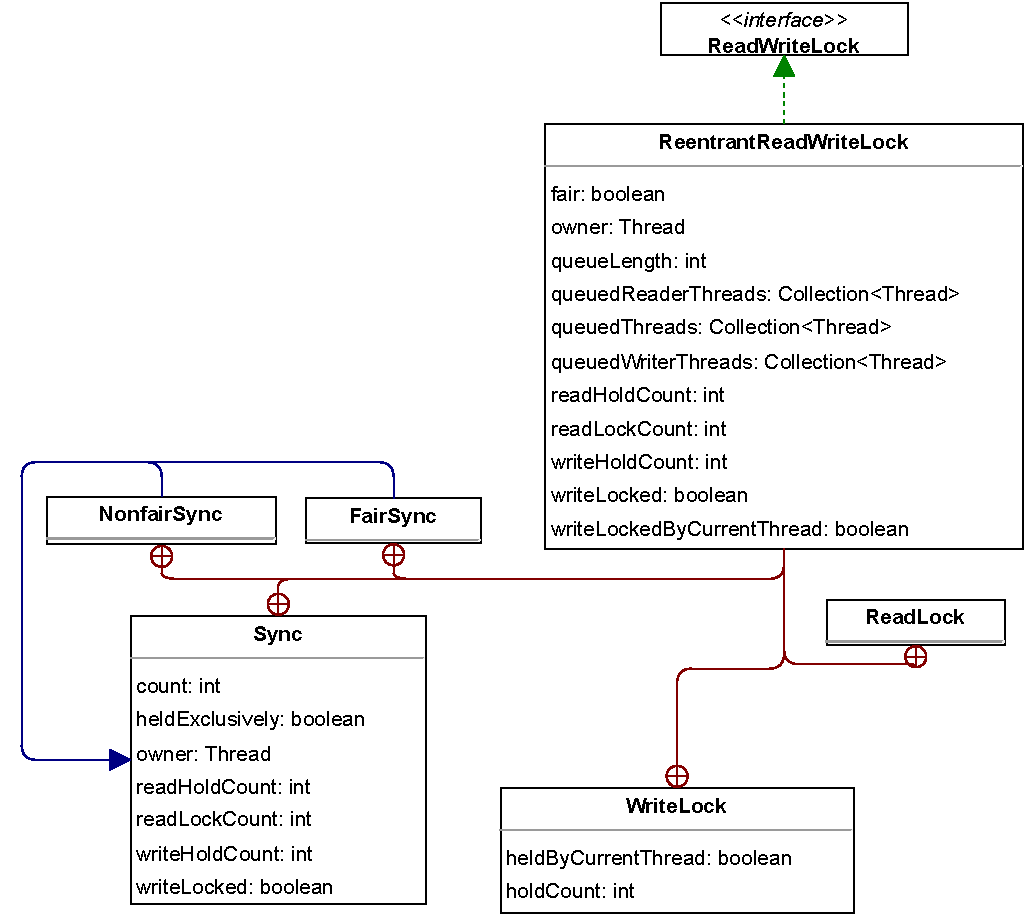
\includegraphics[width=0.7\linewidth]{../../../Images/ReentrantReadWriteLock.pdf}
\end{center}

ReadWriteLock 提供了两个方法,分别用于获取读锁和写锁:

\begin{Java}
public interface ReadWriteLock {
    Lock readLock();
    Lock writeLock();
}
\end{Java}

可以看出,不同于 ReentrantLock 直接实现 Lock 接口,其本身就是一个锁,而 ReentrantReadWriteLock 更像一个管理类,用于控制读锁和写锁。

ReentrantReadWriteLock 内部维护了一个 ReadLock 和一个 WriteLock,他们又依赖 Sync 实现功能。和 ReentrantLock 类似,Sync 也提供了公平锁和非公平锁。

我们知道,AQS 只维护一个 state,而 ReentrantReadWriteLock 需要维护两个锁,怎么办呢? 作为 int 型的 state 拥有 32 位,ReentrantReadWriteLock 将其一分为二,高位表示读状态,低位表示写状态:

\begin{Java}
// Sync
static final int SHARED_SHIFT   = 16;
static final int SHARED_UNIT    = (1 << SHARED_SHIFT);      // 读锁状态值
static final int MAX_COUNT      = (1 << SHARED_SHIFT) - 1;  // 读锁最大值
static final int EXCLUSIVE_MASK = (1 << SHARED_SHIFT) - 1;  // 写锁掩码
static int sharedCount(int c)    { return c >>> SHARED_SHIFT; } // 读锁线程数
static int exclusiveCount(int c) { return c & EXCLUSIVE_MASK; } // 写锁可重入数
\end{Java}

此外,Sync 还记录了首个获取读锁的线程,其重入次数,其他获线程获取读锁的可重入次数等等信息。

\subsubsection*{写锁的获取与释放}

ReentrantReadWriteLock 中的写锁是独占锁,某时只有一个线程可以获取该锁。
\begin{itemize}
    \item 当前没有线程获取读锁和写锁: 可以获取写锁并返回。
    \item 已有线程获取读锁和写锁: 当前请求写锁的线程被阻塞挂起。
\end{itemize}

来看看 tryAcquire 方法:

\begin{Java}
protected final boolean tryAcquire(int acquires) {
    Thread current = Thread.currentThread();
    int c = getState();
    int w = exclusiveCount(c);  // 写锁可重入数
    // c != 0 说明已经有读锁或写锁被获取过
    if (c != 0) {
        // 写锁已被占有 且 不是被当前线程占用
        if (w == 0 || current != getExclusiveOwnerThread())
            return false;
        // 当前线程获取了写锁,重入次数达到上限
        if (w + exclusiveCount(acquires) > MAX_COUNT)
            throw new Error("Maximum lock count exceeded");
        // 重入
        setState(c + acquires);
        return true;
    }
    // 第一个获取写锁的线程
    if (writerShouldBlock() || !compareAndSetState(c, c + acquires))
        return false;
    setExclusiveOwnerThread(current);
    return true;
}
\end{Java}

针对第一个获取写锁的线程,writeShouldBlock 有不同的做法:

\begin{Java}
\\ 非公平锁: 总是 false, 抢占式获取锁
final boolean writerShouldBlock() {
    return false;
}
\\ 公平锁:判断是否有前去节点,有则放弃抢占,进入阻塞队列
final boolean writerShouldBlock() {
    return hasQueuedPredecessors();
}
\end{Java}

可以看出,ReentrantReadWriteLock 殊途同归地使用了和 ReentrantLock 类似的方法。

\subsubsection*{读锁的获取与释放}

获取读锁的过程如下:
\begin{itemize}
    \item 如果没有其他线程持有写锁,则当前线程可以获得读锁,AQS 状态值高 16 位值加一。
    \item 如果其他一个线程持有写锁,当前线程阻塞。
\end{itemize}

来看看 tryAcquireShared 方法:

\begin{Java}
protected final int tryAcquireShared(int unused) {
    Thread current = Thread.currentThread();
    int c = getState();
    // 写锁被占且不是当前线程占用
    if (exclusiveCount(c) != 0 && getExclusiveOwnerThread() != current)
        return -1;
    // 获取读锁计数
    int r = sharedCount(c);
    // 多个线程只有一个会成功获取读锁
    if (!readerShouldBlock() && r < MAX_COUNT && compareAndSetState(c, c + SHARED_UNIT)) {
        // 读锁未被占用过
        if (r == 0) {
            firstReader = current;
            firstReaderHoldCount = 1;
        // 当前线程是第一个获取读锁的线程
        } else if (firstReader == current) {
            firstReaderHoldCount++;
        // 记录最后一个获取读锁的线程或记录其他线程读锁的可重入数
        } else {
            HoldCounter rh = cachedHoldCounter;
            if (rh == null || rh.tid != LockSupport.getThreadId(current))
                cachedHoldCounter = rh = readHolds.get();
            else if (rh.count == 0)
                readHolds.set(rh);
            rh.count++;
        }
        return 1;
    }
    // 获取失败,重试
    return fullTryAcquireShared(current);
}
\end{Java}

如果当前要获取读锁的线程已经持有了写锁,则也可以获取读锁。但是需要注意,当一个线程先获取了写锁,然后获取了读锁处理事情完毕后,要记得把读锁和写锁都释放掉,不能只释放写锁。

\begin{figure}[H]
    \centering
    \small
    \begin{tikzpicture}[scale = 1]
        \node[draw] (lock) at (0,0) {ReentrantReadWriteLock};
        \node[draw] (readLock) at (5,-2) {ReadLock};
        \node[draw] (writeLock) at (5,1) {WriteLock};
        \foreach \y in {2,1,0} {
            \node[draw] (Condition-\y) at (8.5,\y) {Condition};
            \node[draw] (条件队列-\y) at (12,\y) {条件队列};
            \draw[-Stealth] (Condition-\y) -- (条件队列-\y);
            \draw[-Stealth] (writeLock.east) -- (Condition-\y.west);
        }
        \node[draw] (Condition) at (8.5,-2) {Condition};
        \draw [-Stealth] (readLock) -- (Condition);
        \draw [-Stealth] (lock.east) -- (writeLock.west);
        \draw [-Stealth] (lock.east) -- (readLock.west);
        \draw [-Stealth] (lock) -- (AQS);
        \node [draw] (AQS) at (0,-2) {AQS 阻塞队列};
    \end{tikzpicture}
    \caption{ReentrantReadWriteLock}
    \label{fig:ReentrantReadWriteLock}
\end{figure}

\subsection{StampedLock 戳记锁}

\subsubsection*{StampedLock 基础}

StampedLock 是加强版的 ReentrantReadWriteLock, 提供了可操作性更强的功能:

\begin{Java}
public class StampedLock implements java.io.Serializable
\end{Java}

注意,StampedLock 不是基于 AQS 实现的。

StampedLock 提供了三种模式的读写控制,当调用获取锁的系列函数时,会返回一个 long 型变量,称之为 stamp,stamp 代表了锁的状态,stamp 为 0 表示获取锁失败。

\begin{center}
    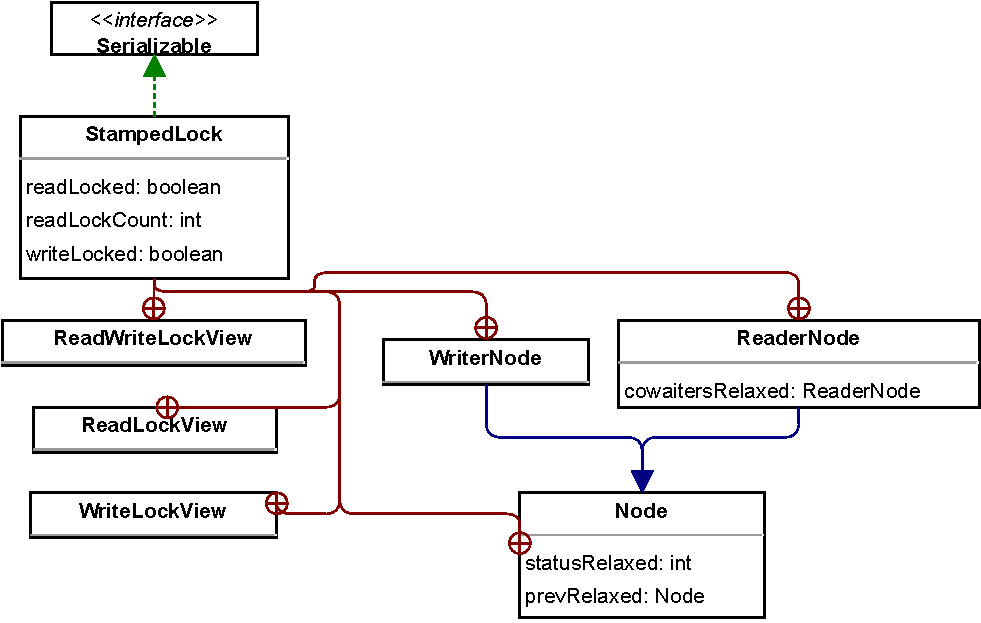
\includegraphics[width=0.7\linewidth]{../../../Images/StampedLock.pdf}
\end{center}

StampedLock 提供的几种读写模式锁分别如下:
\begin{itemize}
    \item \textbf{写锁 writeLock}: 排他/独占锁,和 ReentrantReadWriteLock 读锁最大的不同是不可重入。
    \item \textbf{悲观读锁 readLock}: 共享锁,在没有线程获取独占写锁的情况下,多个线程可以同时获取该锁。如果已经有线程持有写锁,则请求该锁的线程被阻塞。同样不可重入。悲观指的是具体操作数据前会悲观地认为其他线程可能要对自己操作的数据进行修改,所以需要先对数据加锁,这是读少写多情况下地一种考虑。
    \item \textbf{乐观读锁 tryOptimisticRead}: 相对悲观锁来说,在操作数据前并没有通过 CAS 设置锁地状态,仅仅通过位运算测试。如果当前没有线程持有写锁,则简单地返回一个非0的stamp版本信息。
\end{itemize}

由于tryOptimisticRead并没有使用CAS设置锁状态,所以不需要显式地释放该锁。该锁的一个特点是适用于读多写少的场景,因为获取读锁只是使用位操作进行检验,不涉及CAS操作,所以效率会高很多。

但是同时由于没有使用真正的锁,在保证数据一致性上需要复制一份要操作的变量到方法栈,并且在操作数据时可能其他写线程已经修改了数据,而我们操作的是方法栈里面的数据,也就是一个快照,所以最多返回的不是最新的数据,但是一致性还是得到保障的。

StampedLock还支持这三种锁在一定条件下进行相互转换。例如long tryConvertToWriteLock(long  stamp)期望把stamp标记的锁升级为写锁,这个函数会在下面几种情况下返回一个有效的stamp(也就是晋升写锁成功):

\begin{itemize}
    \item 当前锁已经是写锁模式。
    \item 当前锁处于读锁模式,并且没有其他线程是读锁模式。
    \item 当前处于乐观读模式,并且当前写锁可用。
\end{itemize}

\subsubsection*{StampedLock 策略}

StampedLock 通过一个 int 型和 state 和一个队列来实现,对 state 的分割如下:
\begin{itemize}
    \item 高位的 24 位标识版本号,低位的 8 位表示锁。
    \item 低8位第1位表示是否为写锁,剩下7位表示悲观读锁的个数。
\end{itemize}

队列同样使用节点封装线程,采用双向链表实现。

StampedLock 的源码比较复杂,这里只讲三种锁的执行策略:
\begin{itemize}
    \item 写锁的获取与释放
    \begin{itemize}
        \item 获取写锁
        \begin{itemize}
            \item 只有当state的低八位为 0000 0000 的才能申请写锁,即加锁前既没有写锁也没有读锁。
            \item 成功获取锁,state 低八位变成 1000 0000,返回 state 值。
            \item 申请失败,开始自旋,队列不为空直接阻塞,否则有限次数内自旋申请不到就阻塞。
            \item 进入阻塞态,线程被封装为节点进入队尾,如果是第二个节点(第一个为哨兵节点),则开始新一轮自旋。
        \end{itemize}
        \item 释放写锁
        \begin{itemize}
            \item 根据枪锁时返回的 stamp 检验异常。
            \item 没有异常则将 state 版本号 +1,唤醒后继节点抢锁。
        \end{itemize}
    \end{itemize}
    \item 悲观读锁的获取与释放
    \begin{itemize}
        \item 获取读锁
        \begin{itemize}
            \item 如果该锁被另一个线程保持,则阻塞线程,否则自旋申请锁。
            \item 如果申请锁失败,将线程封装为节点 node,此时分两种情况。
            \item 1. 当前尾节点是写锁,则将 node 添加到队尾。等 node 成为第二个节点再开始自旋申请锁。
            \item 2. 当前尾节点是读锁,则将 node 通过名为 cowait 指针与尾结点联系起来,然后阻塞。等尾节点抢锁时,唤醒的线程会通过 cowait 唤醒相关节点来抢锁。
        \end{itemize}
        \item 释放读锁
        \begin{itemize}
            \item 根据枪锁时返回的 stamp 检验异常。
            \item 没有异常则将 state 版本号 +1,唤醒后继节点抢锁。
        \end{itemize}
    \end{itemize}
    \item 乐观读锁: 没有锁,本地线程保存快照进行修改,返回时比较,失败则重试。
\end{itemize}

\begin{figure}[H]
    \centering
    \small
    \begin{tikzpicture}[scale = 1]
        \node[draw] (lock) at (0,0) {StampedLock};
        \node[draw,align=left] (writeLock) at (4,1) {writeLock()};
        \node[draw,align=left] (readLock) at (4,0) {readLock()};
        \node[draw,align=left] (optimisticLock) at (4,-1) {tryOptimisticRead()};
        \node[draw,align=left] (queue) at (0,-2) {双向阻塞队列};
        \draw [-Stealth] (lock) -- (writeLock.west);
        \draw [-Stealth] (lock) -- (readLock.west);
        \draw [-Stealth] (lock) -- (optimisticLock.west);
        \draw [-Stealth] (lock) -- (queue);
        \node[draw] (Condition1) at (8,1) {Condition1};
        \node[draw] (Condition2) at (8,0) {Condition2};
        \node[draw] (Condition3) at (8,-1) {Condition3};
        \draw [-Stealth] (writeLock) -- (Condition1);
        \draw [-Stealth] (readLock) -- (Condition2);
        \draw [-Stealth] (optimisticLock) -- (Condition3);
    \end{tikzpicture}
    \caption{StampedLock}
    \label{fig:StampedLock}
\end{figure}

\newpage